% Volumen diferencial dτ = dx dy dz (libro fig. 2.6)
\documentclass[border=5pt]{standalone}
\usepackage{tikz}
\usetikzlibrary{arrows.meta, calc}
\begin{document}
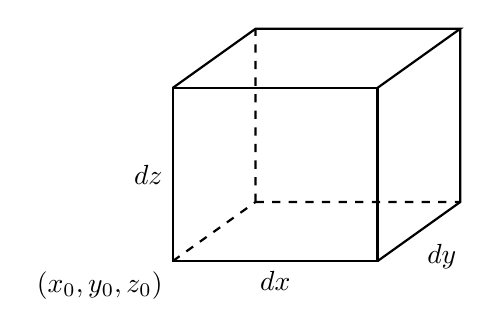
\begin{tikzpicture}[>={Stealth[length=2.4mm]}, line width=0.8pt]
  % proyección: +x=(2.6,0), +y(prof)=(1.05,0.75), +z=(0,2.2)
  \coordinate (A) at (0,0);
  \coordinate (B) at (2.6,0);
  \coordinate (C) at (2.6,2.2);
  \coordinate (D) at (0,2.2);
  \coordinate (A2) at (1.05,0.75);
  \coordinate (B2) at (3.65,0.75);
  \coordinate (C2) at (3.65,2.95);
  \coordinate (D2) at (1.05,2.95);
  % aristas ocultas (desde A2)
  \draw[dashed] (A2)--(B2) (A2)--(D2) (A)--(A2);
  % cara frontal
  \draw (A)--(B)--(C)--(D)--cycle;
  % cara superior y lateral
  \draw (D)--(D2)--(C2)--(C) (B)--(B2)--(C2);
  % etiquetas de aristas
  \node[below] at (1.3,0){$dx$};
  \node[below right] at (3.1,0.35){$dy$};
  \node[left] at (0,1.1){$dz$};
  \node[below left] at (A){$(x_0,y_0,z_0)$};
\end{tikzpicture}
\end{document}
